\FloatBarrier
\section{Methods}
\label{sec:methods}
In this section, accurate methods used to compute the magnetic vector potential~$\mathbf{A}$ and the magnetic field~$\mathbf{B}$
of a straight wire segment and a circular wire loop are presented.
Furthermore, methods to evaluate the magnetostatic quantities in global coordinates are provided.
Particular attention was paid to ensure that the expressions presented in this work
obey the correct asymptotic behavior for evaluation locations
far away from and close to the current carriers.
For most test cases, the full relative accuracy of the floating point
arithmetic chosen for implementation is retained throughout the computations
(16 digits of precision in the IEEE-754 \texttt{binary64}~\cite{ieee754} implementation).
There are a few exceptions where accuracy drops by up to 3 digits of precision
(in the \texttt{binary64} case).
The section concludes with a description of the verification procedure
employed to benchmark these methods.

\FloatBarrier
\subsection{Straight Wire Segment}
\label{sec:methods_sws}
The basic geometry of a single wire segment is shown in Fig.~\ref{fig:straightWireSegment}.
A cylindrical coordinate system~$(\rho, \varphi,z)$ is aligned with the wire segment~(red line),
such that the wire is aligned with the $z$-axis and starts at the origin.
A current $I$ flows along the wire segment of length~$L$ in positive~$z$ direction~(red arrow).
The evaluation point is specified by~$\mathbf{x} = (\rho, \varphi=0, z)$.
$R_\mathrm{i}$ ($R_\mathrm{f}$) denotes the distance from the start (end) of the wire segment to~$\mathbf{x}$.
The angles $\alpha$ and $\beta$ are used in the formulas below.
\begin{figure}[htbp]
 \centering
 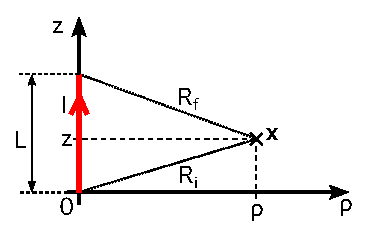
\includegraphics[width=8cm]{img/straightWireSegment.eps}
 \caption{Geometry of a single wire segment (red line) and the associated cylindrical coordinate system.
          The magnetostatic quantities are to be evaluated at a location $\mathbf{x}$.
          After Fig.~1 in Ref.~\cite{hanson_hirshman_2002}.}
 \label{fig:straightWireSegment}
\end{figure}

\subsubsection{Magnetic Vector Potential}
\label{sec:methods_sws_vecpot}
The magnetic vector potential of a straight wire segment
only has component~$A_z$ parallel to the wire:
\begin{equation}
 \mathbf{A} = A_z \hat{\mathbf{e}}_z
\end{equation}
where~$\hat{\mathbf{e}}_z$ is the unit vector in direction $z$.
It is given by~\cite{hanson_hirshman_2002}:
\begin{equation}
  A_z(\rho, z) = \frac{\mu_0 I}{4 \pi} \ln \left( \frac{1 + \epsilon}{1 - \epsilon} \right)
\end{equation}
with
\begin{align}
  \epsilon =&\, \frac{L}{R_\mathrm{i} + R_\mathrm{f}} \\
       R_\mathrm{i} =&\, \sqrt{\rho^2 + z^2} \\
       R_\mathrm{f} =&\, \sqrt{\rho^2 + (1 - z)^2} \, .
\end{align}
In this work normalized coordinates~$\rho' = \rho/L$ and~$z' = z/L$ are used.
This leads to the following expressions
for~$r_\mathrm{i} = R_\mathrm{i}/L$ and~$r_\mathrm{f} = R_\mathrm{f}/L$:
\begin{align}
  r_\mathrm{i} =&\, \sqrt{{\rho'}^2 +      {z'}^2 }       \label{eqn:r_i_default} \\
  r_\mathrm{f} =&\, \sqrt{{\rho'}^2 + (1 - {z'})^2}       \label{eqn:r_f_default} \\
  \Rightarrow
  \epsilon     =&\, \frac{1}{r_\mathrm{i} + r_\mathrm{f}} \label{eqn:eps_default}\, .
\end{align}
For locations on the conductor, $\epsilon = 1$ holds.
The magnetostatic quantites are not defined for evaluation locations on the conductor,
which implies $\epsilon < 1$ for valid evaluation locations.
The value of $\epsilon$ only depends on the sum $r_\mathrm{i} + r_\mathrm{f}$,
which implies that contours of constant $\epsilon$ are ellipses with focii at the ends of the wire segment.
This is similar to the Gardener's construction method for ellipses~\cite{dawson_2021}.
The elliptical contours of constant $\epsilon$ are illustrated in Fig.~\ref{fig:epsilon_contours}.
The contours approach a circular shape far away from the wire segment.
\begin{figure}[htbp]
 \centering
 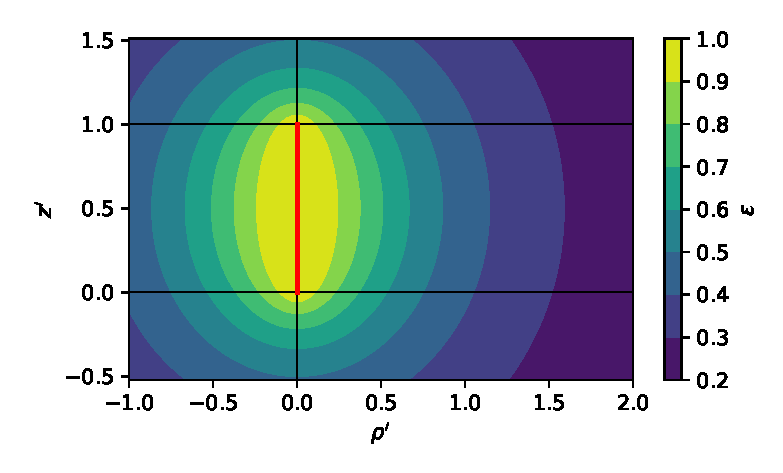
\includegraphics{img/epsilon_contours.eps}
 \caption{Contours of constant $\epsilon$ as computed from \eqn{eps_default}.
          The straight wire segment is located along the red line.}
 \label{fig:epsilon_contours}
\end{figure}
A common prefactor depending on the current~$I$ and~$\mu_0$ is split off:
\begin{equation}
  A_z(\rho', z') = \frac{\mu_0 I}{2 \pi} \tilde{A}_z (\rho', z')
\end{equation}
with
\begin{equation}
  \tilde{A}_z (\rho', z')
  = \frac{1}{2} \ln \left( \frac{1 + \epsilon}{1 - \epsilon} \right)
  = \textrm{atanh} (\epsilon) \, . \label{eqn:A_z_tilde}
\end{equation}
The rest of this section is dedicated to the accurate computation of $\tilde{A}_z (\rho', z')$.
One of several formulations is chosen depending on the evaluation location~$(\rho', z')$:
\begin{equation}
  \tilde{A}_z (\rho', z') =
  \begin{cases}
    \textrm{undefined}                   &:\, \rho' = 0; 0 \leq z' \leq 1 \\
    \tilde{A}_\mathrm{z,ax}  (z')        &:\, \rho' = 0; z' < 0 \textrm{ or } z' > 1  \\
    \tilde{A}_\mathrm{z,rad} (\rho')     &:\, \rho' > 0; z' \in \{0, 1\} \\
    \tilde{A}_\mathrm{z,f}   (\rho', z') &:\, (\rho' \geq 1 \textrm{ and } z' \,\cancel{\in}\, \{0, 1\}) \textrm{ or } \\
                ~                        &~\,\, (\rho' > 0; z' \leq -1 \textrm{ or } z' > 2) \\
    \tilde{A}_\mathrm{z,n}   (\rho', z') &:\, \textrm{elsewhere} \, .
  \end{cases} \label{eqn:sws_A_z_switchover}
\end{equation}
The domain decomposition for the accurate computation of $\tilde{A}_z$
formulated in \eqn{sws_A_z_switchover} is illustrated in Fig.~\ref{fig:sws_regions}(a).
For the case~$\rho'=0$, the following formulation is used:
\begin{equation}
  \tilde{A}_\mathrm{z,ax} (z') =
  \begin{cases}
    \tilde{A}_\mathrm{z,ax,f} (z') &:\, z' < -1 \textrm{ or } z' \geq 2 \\
    \tilde{A}_\mathrm{z,ax,n} (z') &:\, -1 \leq z' < 0 \textrm{ or } 1 < z' < 2
  \end{cases}
\end{equation}
with
\begin{equation}
  \tilde{A}_\mathrm{z,ax,f} (z') = \textrm{atanh}\left( \frac{1}{|z'| + |1 - z'|} \right) \label{eqn:sws_A_z_ax_f}
\end{equation}
(derived in \eqn{sws_A_z_ax_f_derivation})
and
\begin{equation}
  \tilde{A}_\mathrm{z,ax,n} (z') = \frac{1}{2} \frac{z'}{|z'|} \ln \left(\frac{z'}{z' - 1}\right) \label{eqn:sws_A_z_ax_n} \, ,
\end{equation}
which is derived in \eqn{sws_A_z_ax_n_derivation}.
The cases with $z'=0$ or $z'=1$ are evaluated using the following expressions:
\begin{equation}
  \tilde{A}_\mathrm{z,rad} (\rho') =
  \begin{cases}
    \tilde{A}_\mathrm{z,rad,f} (\rho') &:\, \rho' > 1 \\
    \tilde{A}_\mathrm{z,rad,n} (\rho') &:\, 0 < \rho' \leq 1
  \end{cases}
\end{equation}
with
\begin{equation}
  \tilde{A}_\mathrm{z,rad,f} (\rho') = \textrm{atanh}\left( \frac{1}{\rho' + \sqrt{{\rho'}^2 + 1}} \right) \label{eqn:sws_A_z_rad_f}
\end{equation}
(derived in \eqn{sws_A_z_rad_f_derivation})
and
\begin{equation}
  \tilde{A}_\mathrm{z,rad,n} (\rho') = \frac{1}{2} \ln \left(\frac{\rho' c + 1 + c}{\rho' c + 2 s^2 }\right) \label{eqn:sws_A_z_rad_n}
\end{equation}
where
\begin{align}
  c =&\, \frac{1}{\sqrt{{\rho'}^2 + 1}} \\
  s =&\, \sin(\arctan(\rho')/2) \, .
\end{align}
The derivation for this formulation can be found in \eqn{sws_A_z_rad_n_derivation}.
The case of~$\tilde{A}_\mathrm{z,f}(\rho', z')$ is the straight-forward implementation of:
\begin{equation}
  \tilde{A}_\mathrm{z,f}(\rho', z') = \textrm{atanh} (\epsilon)
\end{equation}
with~$r_\mathrm{i}$, $r_\mathrm{f}$ and~$\epsilon$ from~\eqn{r_i_default}, \eqn{r_f_default} and~\eqn{eps_default}, respectively.
For all other permitted locations, the following evaluation is used:
\begin{equation}
  \tilde{A}_\mathrm{z,n} (\rho', z') = \frac{1}{2} \left[ \ln\left(n + 1 \right) - \ln \left( n \right)  \right] \label{eqn:sws_A_z_n}
\end{equation}
with
\begin{align}
  n                       =&\, r_\mathrm{i} \sin^2(\alpha/2) + r_\mathrm{f} \sin^2(\beta/2) \\
  \alpha =&\, \texttt{atan2}(\rho', z')   \label{eqn:sws_alpha} \\
  \beta  =&\, \texttt{atan2}(\rho', 1-z') \label{eqn:sws_beta}
\end{align}
and~$r_\mathrm{i}$, $r_\mathrm{f}$ from~\eqn{r_i_default}, \eqn{r_f_default}, respectively.
Trigonometric functions are used here since they offer increased numerical robustness
for the evaluation locations under consideration in this case.
The derivation for this formulation is found in the appendix around \eqn{sws_A_z_n_derivation}.

\subsubsection{Magnetic Field}
\label{sec:methods_sws_magfld}
The magnetic field of a straight wire segment
is given by the law of Biot and Savart as follows~\cite{hanson_hirshman_2002}:
\begin{equation}
 \mathbf{B}
 = \frac{\mu_0 I}{4 \pi}
   \hat{\mathbf{e}}_z \times \mathbf{R}_\mathrm{i}
   \frac{2 L (R_\mathrm{i} + R_\mathrm{f})}{R_\mathrm{i} R_\mathrm{f}} \frac{1}{\left(R_\mathrm{i} + R_\mathrm{f}\right)^2 - L^2} \, . \label{eqn:sws_B_phi}
\end{equation}
The vector~$\mathbf{R}_\mathrm{i}$ has components in directions parallel~($z$) and perpendicular~($\rho$) to the wire segment:
\begin{equation}
 \mathbf{R}_\mathrm{i}
 = z \,\hat{\mathbf{e}}_z + \rho \,\hat{\mathbf{e}}_\rho \label{eqn:R_i_vec}
\end{equation}
where $\rho$ and $z$ are cylindrical coordinates in the coordinate system aligned with the wire segment.
The vector-valued term in~\eqn{sws_B_phi} is reformulated as follows by inserting \eqn{R_i_vec}:
\begin{align}
 \hat{\mathbf{e}}_z \times \mathbf{R}_\mathrm{i}
 =&\, \hat{\mathbf{e}}_z \times \left( z \,\hat{\mathbf{e}}_z + \rho \,\hat{\mathbf{e}}_\rho \right) \nonumber \\
 =&\,      z \underbrace{\hat{\mathbf{e}}_z \times \hat{\mathbf{e}}_z}_{=0}
      + \rho \underbrace{\hat{\mathbf{e}}_z \times \hat{\mathbf{e}}_\rho}_{=\hat{\mathbf{e}}_\varphi}
 = \rho \,\hat{\mathbf{e}}_\varphi \, .
\end{align}
It follows that the magnetic field of a straight wire segment only has a component~$B_\varphi$ in tangential~($\varphi$) direction:
\begin{equation}
 \mathbf{B} = B_\varphi \hat{\mathbf{e}}_\varphi
\end{equation}
with
\begin{equation}
 B_\varphi (\rho, z)
 = \frac{\mu_0 I}{4 \pi}
   \frac{2 \rho L (R_\mathrm{i} + R_\mathrm{f})}{R_\mathrm{i} R_\mathrm{f}}
   \frac{1}{\left(R_\mathrm{i} + R_\mathrm{f}\right)^2 - L^2} \, .
\end{equation}
This is now reformulated to use normalized coordinates
(as done above for the computation of the magnetic vector potential):
\begin{equation}
 B_\varphi(\rho', z')
 = \frac{\mu_0 I}{4 \pi L}
   \left(\frac{1}{r_\mathrm{f}} + \frac{1}{r_\mathrm{i}} \right)
   \frac{2 \rho'}{\left( r_\mathrm{i} + r_\mathrm{f} \right)^2 - 1} \, .
\end{equation}
Again a normalization factor is split off:
\begin{equation}
  B_\varphi(\rho', z') = \frac{\mu_0 I}{4 \pi L} \tilde{B}_\varphi(\rho', z')
\end{equation}
with
\begin{equation}
  \tilde{B}_\varphi(\rho', z')
  = \left(\frac{1}{r_\mathrm{f}} + \frac{1}{r_\mathrm{i}} \right)
    \frac{2 \rho'}{\left( r_\mathrm{i} + r_\mathrm{f} \right)^2 - 1} \, .
\end{equation}
Consider the denominator in more detail:
\begin{align}
 \left(r_\mathrm{i} + r_\mathrm{f}\right)^2 - 1
 =&\, r_\mathrm{i}^2 + 2 r_\mathrm{i} r_\mathrm{f} + r_\mathrm{f}^2 - 1 \nonumber \\
 =&\, {\rho'}^2 + {z'}^2 + 2 r_\mathrm{i} r_\mathrm{f} + {\rho'}^2 + (1 - z')^2 - 1 \nonumber \\
 =&\, {\rho'}^2 + {z'}^2 + 2 r_\mathrm{i} r_\mathrm{f} + {\rho'}^2 \bcancel{+ 1} - 2 z' + {z'}^2 \bcancel{- 1} \nonumber \\
 =&\, 2 {\rho'}^2 + 2 {z'}^2 + 2 r_\mathrm{i} r_\mathrm{f} - 2 z' \nonumber \\
 =&\, 2 \left[ {\rho'}^2 + r_\mathrm{i} r_\mathrm{f} - z' (1 - z') \right] \, .
\end{align}
This leads to:
\begin{equation}
 \tilde{B}_\varphi(\rho', z')
  = \left(\frac{1}{r_\mathrm{f}} + \frac{1}{r_\mathrm{i}} \right)
    \frac{\bcancel{2} \rho'}{\bcancel{2} \left[ {\rho'}^2 + r_\mathrm{i} r_\mathrm{f} - z' (1 - z') \right]} \, . \label{eqn:bPhiTilde}
\end{equation}
One of several formulations is chosen depending on the evaluation location~$(\rho', z')$:
\begin{equation}
  \tilde{B}_\varphi (\rho', z') =
  \begin{cases}
    \textrm{undefined}                           &:\, \rho' = 0; 0 \leq z' \leq 1 \\
    0                                            &:\, \rho' = 0; z' < 0 \textrm{ or } z' > 1 \\
    \tilde{B}_{\varphi,\mathrm{rad}} (\rho')     &:\, \rho' > 0; z' \in \{0, 1\} \\
    \tilde{B}_{\varphi,\mathrm{f}}   (\rho', z') &:\, (\rho' > 0; z' > 1 \textrm{ or } z' < 0) \textrm{ or } \\
                                            ~    &~~  (\rho' \geq z' \textrm{ or } \rho' \geq 1-z'; 0 < z' < 1) \\
    \tilde{B}_{\varphi,\mathrm{n}}   (\rho', z') &:\, \textrm{elsewhere} \, .
  \end{cases} \label{eqn:sws_B_phi_switchover}
\end{equation}
The domain decomposition for the accurate computation of $\tilde{B}_\varphi$
formulated in \eqn{sws_B_phi_switchover} is illustrated in Fig.~\ref{fig:sws_regions}(b).
The special case~$z' \in \{0, 1\}$ for $\rho'>0$ is implemented as follows:
\begin{equation}
  \tilde{B}_{\varphi,\mathrm{rad}} (\rho') = \frac{1}{\rho' \sqrt{{\rho'}^2 + 1}} \label{eqn:sws_B_phi_rad} \, .
\end{equation}
The derivation of this formulation is found in \eqn{sws_B_phi_rad_derivation}.
The formula in~\eqn{bPhiTilde} is used for evaluation locations far away from the wire
as well as a part of the near-field close to the wire segment:
\begin{equation}
  \tilde{B}_{\varphi,\mathrm{f}} (\rho', z')
  = \left(\frac{1}{r_\mathrm{f}} + \frac{1}{r_\mathrm{i}} \right)
    \frac{\rho'}{{\rho'}^2 + r_\mathrm{i} r_\mathrm{f} - z' (1 - z')} \, .
\end{equation}
For all other permitted locations the following evaluation is used:
\begin{equation}
  \tilde{B}_{\varphi,\mathrm{n}} (\rho', z')
  = \left(\frac{1}{r_\mathrm{f}} + \frac{1}{r_\mathrm{i}} \right)
    \frac{\rho'}
         {{\rho'}^2 + 2 r_\mathrm{i} \left[ r_\mathrm{f} \sin^2(\beta/2) + (1 - z') \sin^2(\alpha/2) \right]} \label{eqn:sws_B_phi_n}
\end{equation}
with~$\alpha$ and~$\beta$ from~\eqn{sws_alpha} and~\eqn{sws_beta}, respectively.
The derivation of this formulation is given in \eqn{sws_B_phi_n_derivation}.
\begin{figure}[htbp]
    \centering
    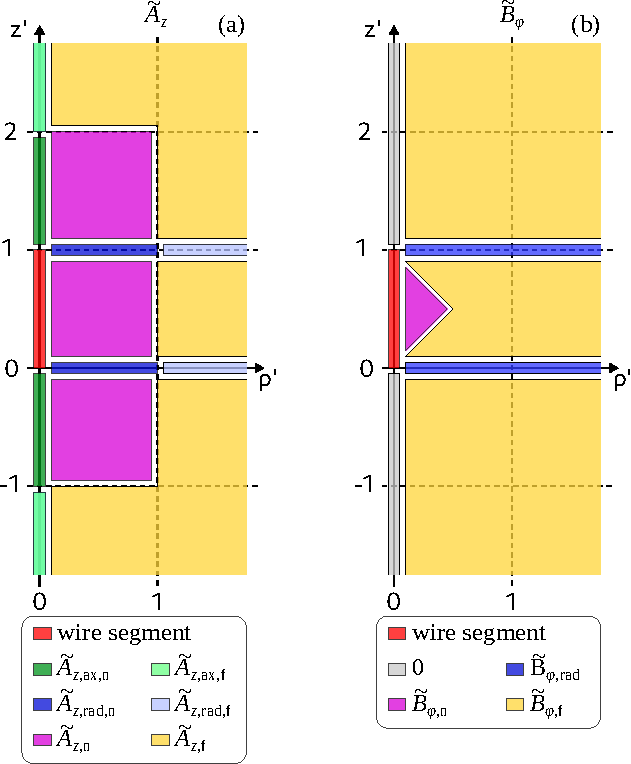
\includegraphics{img/sws_regions.pdf}
    \caption{Domain decomposition used to partition the evaluation region
             for computing $\tilde{A}_z$ (a) and $\tilde{B}_\varphi$ (b) accurately.
             The colored regions indicate at which evaluation locations $(\rho',z')$
             which formulation (see legend) is used.}
    \label{fig:sws_regions}
\end{figure}

\FloatBarrier
\subsection{Circular Wire Loop}
\label{sec:methods_cwl}
The basic geometry of a circular wire loop under consideration here is shown in Fig.~\ref{fig:circularWireLoop}.
The loop is centered at the origin with its normal vector aligned with the $z$-axis.
The radius of the loop is denoted $a$ and a current $I$ (with corresponding current density~$\mathbf{j}$)
flows in the direction indicated in Fig.~\ref{fig:circularWireLoop}.
The magnetic field and vector potential are to be evaluated at the point $\mathbf{x}$ in the ($x$, $z$)-plane.
The coordinates of the evaluation point can be expressed in spherical coordinates as~$(r, \theta)$
or in cylindrical coordinates as~$(\rho, z)$.
The axisymmetry of this setup always allows to rotate the coordinate system such that $\varphi=0$ can be assumed.
\begin{figure}[htbp]
 \centering
 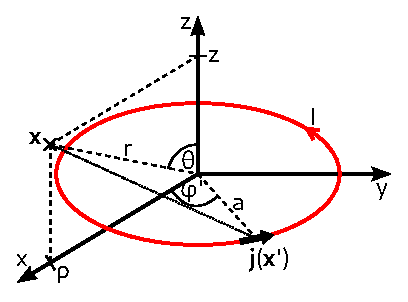
\includegraphics[width=0.5\textwidth]{img/circularWireLoop.eps}
 \caption{Geometry of a circular wire loop centered at the origin with normal vector aligned with the $z$-axis.}
 \label{fig:circularWireLoop}
\end{figure}
Similar to the case of the straight wire segment,
the magnetic vector potential and the magnetic field of the circular wire loop
are assembled from various formulations for special cases of the far-field and the near-field
in the implementation described later.

\subsubsection{Magnetic Vector Potential}
The magnetic vector potential of a circular wire loop
only has a tangential component~$A_\varphi$.
In Eqn.~(5.37) of Ref.~\cite{jackson}, $A_\varphi$~is expressed as
follows for a loop of radius~$a$ and current~$I$ along it:
\begin{align}
  A_\varphi(r, \theta) &= \frac{\mu_0}{4 \pi}
                          \frac{4 I a}{\sqrt{a^2 + r^2 + 2 a r \sin(\theta)}}
                          \left[
                            \frac{(2 - k^2)\mathcal{K}(k) - 2 \mathcal{E}(k)}{k^2}
                          \right] \label{eqn:cwl_A_phi_Jackson}
\end{align}
with
\begin{equation}
  k^2 = \frac{4 a r \sin(\theta)}{a^2 + r^2 + 2 a r \sin(\theta)} \, .
\end{equation}
Here, $\mathcal{K}(k)$ and $\mathcal{E}(k)$ are the complete elliptic integrals of the first and second kind, respectively.
Spherical coordinates~$(r, \theta)$ are used to specify the evaluation location.
The corresponding cylindrical coordinates~$(\rho, z)$ are given by
$\rho = r \sin(\theta)$ and $z = \sqrt{r^2 - \rho^2}$.
Normalized coordinates~$(\rho', z')$ are introduced with
\begin{align}
  \rho' =&\, \rho / a \label{eqn:rhoP} \\
    z'  =&\,   z  / a \label{eqn:zP}   \, .
\end{align}
An expression for the linear combination of $\mathcal{K}(k)$ and $\mathcal{E}(k)$
is used to reformulate \eqn{cwl_A_phi_Jackson}:
\begin{equation}
  \lambda \mathcal{K}(k) + \mu \mathcal{E}(k) = \,\mathrm{cel}(k_c, 1, \lambda + \mu, \lambda + \mu k_c^2) \label{eqn:K_E_by_cel}
\end{equation}
where
\begin{equation}
  k_\mathrm{c}^2 = 1 - k^2
\end{equation}
and cel is the so-called general complete elliptic integral
introduced by Bulirsch~\cite{bulirsch_3}:
\begin{equation}
  \mathrm{cel}(k_c, p, a, b) =
  \int\limits_0^{\pi/2}
    \frac{a \cos^2(\varphi) + b \sin^2(\varphi)}
         {\cos^2(\varphi) + p \sin^2(\varphi)}
    \frac{\mathrm{d}\varphi}
         {\sqrt{\cos^2(\varphi) + k_c^2 \sin^2(\varphi)}} \, .
\end{equation}
The argument of the elliptic integrals is considered first:
\begin{align}
  k^2 &= \frac{4 a r \sin(\theta)}{a^2 + r^2 + 2 a r \sin(\theta)}
       = \frac{4 a \rho}{a^2 + r^2 + 2 a \rho}
       = \frac{4 \bcancel{a} \rho}{a^{\bcancel{2}} \left(1 + \frac{r^2}{a^2} + 2 \frac{\rho}{a} \right)} \nonumber \\
  ~   &= \frac{4 \rho'}{1 + \frac{r^2}{a^2} + 2 \rho'}
       = 4 \rho' \left( 1 + \frac{\rho^2 + z^2}{a^2} + 2 \rho' \right)^{-1} \nonumber \\
  ~   &= 4 \rho' \left( 1 + \rho'^{2} + z'^{2} + 2 \rho' \right)^{-1}
       = \frac{4 \rho'}{z'^2 + (1 + \rho')^2} \, . \label{eqn:kSq}
\end{align}
This implies:
\begin{equation}
  k_c^2 = \frac{z'^2 + (1 - \rho')^2}{z'^2 + (1 + \rho')^2} \, . \label{eqn:kCSq_general}
\end{equation}
The coefficients of the elliptic integrals in \eqn{cwl_A_phi_Jackson} are identified as follows:
\begin{align}
  \lambda &= \frac{2 - k^2}{k^2} = \frac{2}{k^2} - 1 \\
  \mu     &= -\frac{2}{k^2}
\end{align}
and their combinations are as follows for use in \eqn{K_E_by_cel}:
\begin{align}
  \lambda + \mu       &= \frac{2}{k^2} - 1 - \frac{2}{k^2}     = -1 \\
  \lambda + \mu k_c^2 &= \frac{2}{k^2} - 1 - \frac{2}{k^2} (1 - k^2) \nonumber \\
          ~           &= \frac{2}{k^2} - 1 - \frac{2}{k^2} + 2 =  1 \label{eqn:lmkcsq} \, .
\end{align}
Putting Eqn.s~(\ref{eqn:K_E_by_cel}) to~(\ref{eqn:lmkcsq}) together, we arrive at the following expression for $A_\varphi$:
\begin{equation}
 A_\varphi(\rho', z') = \frac{\mu_0 I}{\pi}
                        \frac{1}{\sqrt{z'^2 + (1 + \rho')^2}} \,\mathrm{cel}(k_c, 1, -1, 1) \, . \label{eqn:cwl_A_phi_cel}
\end{equation}
It is favorable for numerical evaluation of $A_\varphi$ to use the form given in \eqn{cwl_A_phi_cel}
where the linear combination of the complete elliptic integrals is embedded in the parameters of cel
and less precautions need to be taken to deal with cancellations in \eqn{cwl_A_phi_Jackson}.
A physics-oriented prefactor is split off to be able to focus on geometry in the following:
\begin{equation}
  A_\varphi(\rho', z') = \frac{\mu_0 I}{\pi} \tilde{A}_\varphi(\rho',z') \label{eqn:norm_A_phi}
\end{equation}
with
\begin{equation}
  \tilde{A}_\varphi(\rho',z')
  = \frac{1}{\sqrt{z'^2 + (1 + \rho')^2}} \,\mathrm{cel}(k_c, 1, -1, 1) \, .
\end{equation}
One of several formulations for $\tilde{A}_\varphi$ is chosen depending on the evaluation location~$(\rho', z')$:
\begin{equation}
  \tilde{A}_\varphi (\rho', z') =
  \begin{cases}
    0                                          &:\, \rho' = 0 , \textrm{ any } z' \\
    \tilde{A}_{\varphi,\mathrm{f}} (\rho', z') &:\, 0 < \rho' < 1/2 \textrm{ or } \rho' > 2 \textrm{ or } |z'| \geq 1 \\
    \tilde{A}_{\varphi,\mathrm{n}} (\rho', z') &:\, 1/2 \leq \rho' \leq 2 \textrm{ but } \rho' \neq 1, |z'| < 1 \\
    \tilde{A}_{\varphi,\mathrm{v}} (z')        &:\, \textrm{else } (\rho' = 1, |z'| < 1) \, .
  \end{cases} \label{eqn:A_phi_final}
\end{equation}
The domain decomposition used to compute $\tilde{A}_\varphi$ accurately is depicted in Fig.~\ref{fig:cwl_A_phi_regions}.
\begin{figure}[htbp]
    \centering
    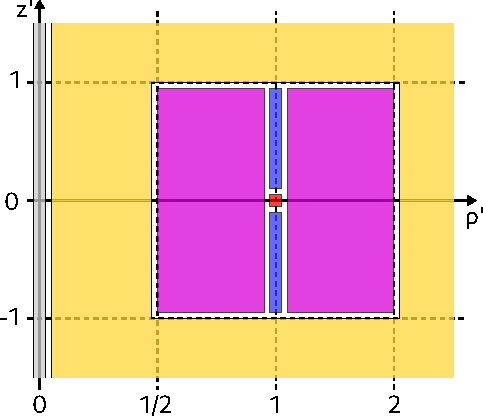
\includegraphics{img/cwl_A_phi_regions.pdf}
    \caption{Domain decomposition used to partition the evaluation region
             for computing $\tilde{A}_\varphi$ accurately.
             The colored regions indicate at which evaluation locations $(\rho',z')$
             which formulation (see legend) is used.}
    \label{fig:cwl_A_phi_regions}
\end{figure}
The following formula is implemented for evaluation locations away from the wire loop:
\begin{equation}
  \tilde{A}_{\varphi,\mathrm{f}} (\rho',z')
  = \frac{k^2}{\sqrt{z'^2 + (1 + \rho')^2}} \,\mathcal{C}(k_c) \label{eqn:cwl_A_phi_f}
\end{equation}
with $k^2$~from~\eqn{kSq} and
\begin{equation}
  \mathcal{C}(k_c)
  = \,\mathrm{cel} \left( \frac{2 \sqrt{k_c}}{1 + k_c}, 1, 0, \frac{2}{(1 + k_c)^3} \right) \, . \label{eqn:elliptic_c}
\end{equation}
Close to the wire loop, the following formulation is used:
\begin{equation}
  \tilde{A}_{\varphi,\mathrm{n}} (\rho',z')
  = \frac{1}{|\rho' - 1| \sqrt{\left( \frac{z'}{\rho'-1} \right)^2 + \left(1 + \frac{2}{\rho'-1} \right)^2 }}
    \,\mathrm{cel}(\sqrt{k_c^2}, 1, -1, 1) \label{eqn:cwl_A_phi_n}
\end{equation}
with $k_c^2$ computed as follows:
\begin{equation}
  k_c^2 = \frac{\left( \frac{z'}{\rho'-1} \right)^2 + 1}{\left( \frac{z'}{\rho'-1} \right)^2 + \left(1 + \frac{2}{\rho'-1} \right)^2} \, .
\end{equation}
At~$\rho' = 1$, some further simplification can be carried out.
This leads to the following formulation for~$\rho' = 1$ and~$|z'| < 1$:
\begin{equation}
  \tilde{A}_{\varphi,\mathrm{v}} (z') = \frac{1}{|z'|} \,\mathrm{cel}\left(\frac{1}{k_c}, 1, 1, -1\right) \label{eqn:cwl_A_phi_v}
\end{equation}
with $k_c$ computed as follows:
\begin{equation}
  k_c = \frac{|z'|}{\sqrt{4 + {z'}^2}} \, .
\end{equation}

\subsubsection{Magnetic Field}
The magnetic field produced by a circular wire loop is made up of two components:
\begin{equation}
  \mathbf{B} = B_\rho \hat{\mathbf{e}}_\rho + B_z \hat{\mathbf{e}}_z
\end{equation}
where $B_\rho$ denotes the radial component and $B_z$ denotes the vertical component.
The radial component~$B_\rho$ is given by~\cite{teal}:
\begin{equation}
  B_\rho(\rho', z')
  = \frac{\mu_0 I}{\pi a} \frac{z'}{\left[ z'^2 + (1 + \rho')^2 \right]^{3/2}} \,\mathrm{cel}(k_c, k_c^2, -1, 1)
\end{equation}
Also here, a normalization factor is split off:
\begin{equation}
  B_\rho(\rho', z') = \frac{\mu_0 I}{\pi a} \tilde{B}_\rho(\rho', z')
\end{equation}
with
\begin{align}
  \tilde{B}_\rho(\rho', z')
  =&\, \frac{z'}{\left[ z'^2 + (1 + \rho')^2 \right]^{3/2}} \,\mathrm{cel}(k_c, k_c^2, -1, 1) \, .
\end{align}
One of several formulations is chosen depending on the evaluation location~$(\rho', z')$:
\begin{equation}
  \tilde{B}_\rho(\rho', z')
  = \begin{cases}
      0                                 &:\, \rho' = 0, \textrm{ any } z' \\
                    ~                   &\, ~\textrm{ or } \rho' > 0, z' = 0 \\
      \tilde{B}_{\rho,\mathrm{f}} (\rho', z') &:\, \rho' < 1/2 \textrm{ or } \rho' > 2 \textrm{ or } |z'| \geq 1 \\
      \tilde{B}_{\rho,\mathrm{n}} (\rho', z') &:\, 1/2 \leq \rho' \leq 2 \textrm{ but } \rho' \neq 1, |z'| < 1 \\
      \tilde{B}_{\rho,\mathrm{v}} (z')        &:\, \textrm{else } (\rho' = 1, |z'| < 1) \, .
    \end{cases} \label{eqn:cwl_B_rho_switchover}
\end{equation}
The domain decomposition used to compute $\tilde{B}_\rho$ accurately is depicted in Fig.~\ref{fig:cwl_B_rho_regions}.
\begin{figure}[htbp]
    \centering
    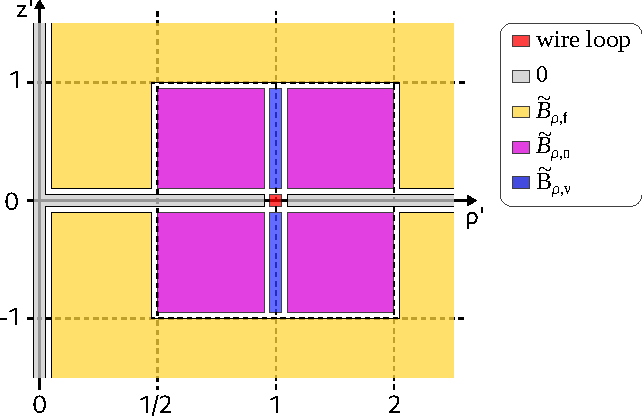
\includegraphics{img/cwl_B_rho_regions.pdf}
    \caption{Domain decomposition used to partition the evaluation region
             for computing $\tilde{B}_\rho$ accurately.
             The colored regions indicate at which evaluation locations $(\rho',z')$
             which formulation (see legend) is used.}
    \label{fig:cwl_B_rho_regions}
\end{figure}
The following formulation is implemented for evaluation locations away from to the wire loop:
\begin{equation}
  \tilde{B}_{\rho,\mathrm{f}} (\rho', z')
  = \frac{4 \rho' z' \left[ \,\mathcal{D}(k_c) - \,\mathcal{C}(k_c) \right]}
         {\left[{z'}^2 + (1 + \rho')^2 \right]^{3/2} \left[{z'}^2 + (1 - \rho')^2 \right] } \label{eqn:cwl_B_rho_f}
\end{equation}
with
\begin{equation}
  \mathcal{D}(k_c)
  = \frac{\mathcal{K}(k) - \,\mathcal{E}(k)}{k^2}
  = \,\mathrm{cel}(k_c, 1, 0, 1) \, . \label{eqn:elliptic_d}
\end{equation}
For points close to the wire loop, but with~$\rho' \neq 1$, the following formulation is used:
\begin{align}
  \tilde{B}_{\rho,\mathrm{n}}& (\rho', z')
  = \frac{4 \rho' \left|\frac{z'}{\rho'-1}\right| \left[ \,\mathcal{D}(k_c) - \,\mathcal{C}(k_c) \right]}
         {(\rho' - 1)^4} \nonumber \\
  ~& \left\{
      \left[ \left( \frac{z'}{\rho'-1} \right)^2 + \left(1 + \frac{2}{\rho'-1} \right)^2 \right]^{3/2}
      \left[ \left( \frac{z'}{\rho'-1} \right)^2 + 1 \right]
    \right\}^{-1} \label{eqn:cwl_B_rho_n} \, .
\end{align}
Finally, for $\rho'=1$ and~$|z'| < 1$, the following formulation is used:
\begin{equation}
  \tilde{B}_{\rho,\mathrm{v}} (z')
  = \frac{k_c}{2} \frac{z'}{|z'|} \left[ \left( \frac{2}{z'^2} + 1 \right) \mathcal{E}(k_c) - \mathcal{K}(k_c) \right] \label{eqn:cwl_B_rho_v}
\end{equation}
with
\begin{equation}
  k_c^2 = \frac{1}{1 + 4/{z'}^2}
\end{equation}
and
\begin{align}
  \mathcal{K}(k_c) =&\, \,\mathrm{cel}(k_c, 1, 1, 1) \\
  \mathcal{E}(k_c) =&\, \,\mathrm{cel}(k_c, 1, 1, k_c^2) \, .
\end{align}
The vertical component~$B_z$ of the magnetic field of a circular wire loop is given by~\cite{teal}:
\begin{align}
 B_z(\rho', z')
 =&\, \frac{\mu_0 I}{2 \pi a}
   \frac{1}{\rho' \sqrt{z'^2 + (1 + \rho')^2}} \nonumber \\
 ~& \left[
       \textrm{cel}(k_c, 1, -1, 1)
     + \frac{1 + k_c^2 - \left( 1 - k_c^2 \right) \rho'}{2} \textrm{cel}(k_c, k_c^2, -1, 1)
   \right]
\end{align}
A normalization factor is split off here as well:
\begin{equation}
  B_z(\rho', z') = \frac{\mu_0 I}{\pi a} \tilde{B}_z(\rho', z')
\end{equation}
with
\begin{align}
  \tilde{B}_z(\rho', z')
  =&\, \frac{1}{2 \rho' \sqrt{z'^2 + (1 + \rho')^2}} \nonumber \\
 ~& \left[
       \textrm{cel}(k_c, 1, -1, 1)
     + \frac{1 + k_c^2 - \left( 1 - k_c^2 \right) \rho'}{2} \textrm{cel}(k_c, k_c^2, -1, 1)
   \right] \, .
\end{align}
The evaluation of this formula is split up as well into separate special cases.
One of several formulations is selected depending on the evaluation location~$(\rho', z')$:
\begin{equation}
  \tilde{B}_z(\rho', z')
  = \begin{cases}
      \tilde{B}_{z,\mathrm{f1}} (\rho', z') &:\, \rho' < 1/2, \textrm{ any } z' \\
                ~                           &~ \textrm{ or } \rho' \leq 2, |z'| > 1 \\
      \tilde{B}_{z,\mathrm{f2}} (\rho', z') &:\, \rho' > 2, \textrm{ any } z' \\
      \tilde{B}_{z,\mathrm{n}}  (\rho', z') &:\, 1/2 \leq \rho' \leq 2 \textrm{ but } \rho' \neq 1, |z'| \leq 1 \\
      \tilde{B}_{z,\mathrm{v}}  (z') &:\, \textrm{else } (\rho' = 1, |z'| \leq 1) \, .
    \end{cases} \label{eqn:cwl_B_z_switchover}
\end{equation}
The domain decomposition used to compute $\tilde{B}_z$ accurately is depicted in Fig.~\ref{fig:cwl_B_z_regions}.
\begin{figure}[htbp]
    \centering
    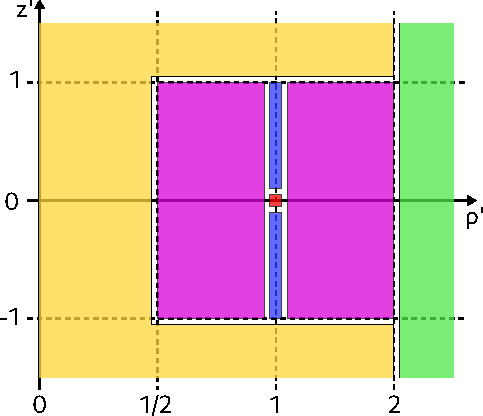
\includegraphics{img/cwl_B_z_regions.pdf}
    \caption{Domain decomposition used to partition the evaluation region
             for computing $\tilde{B}_z$ accurately.
             The colored regions indicate at which evaluation locations $(\rho',z')$
             which formulation (see legend) is used.}
    \label{fig:cwl_B_z_regions}
\end{figure}
For points not too close to the wire loop and with $\rho' \leq 2$, the following formulation is used:
\begin{align}
  \tilde{B}_{z,\mathrm{f1}} (\rho', z')
  =&\, \frac{1}{\sqrt{{z'}^2 + (1+\rho')^2} \left[{z'}^2 + (1 - \rho')^2 \right] } \nonumber \\
  ~&\,  \left\{ \mathcal{E}(k_c) + \rho' \left[ \mathcal{E}(k_c) - 2 \mathcal{K}(k_c) + 2 \mathcal{D}(k_c) \right] \right\} \, . \label{eqn:cwl_B_z_f1}
\end{align}
A second far-field method is needed for points with $\rho' > 2$:
\begin{equation}
  \tilde{B}_{z,\mathrm{f2}} (\rho', z')
  = \frac{1}{\sqrt{t_1 + t_2}(t_1-t_2) {\rho'}^3}
    \left\{ \mathcal{E}(k_c) + \frac{4}{\alpha_\mathrm{cd}} \left[ \mathcal{C}(k_c) - \,\mathcal{D}(k_c) \right] \right\} \label{eqn:cwl_B_z_f2}
\end{equation}
with
\begin{align}
  t_1 =&\, \frac{z'^2 + 1}{\rho'^2} + 1 \\
  t_2 =&\, \frac{2}{\rho'}
\end{align}
and
\begin{equation}
  \alpha_\mathrm{cd} = 1 + \frac{1}{\rho'} \left[ 2 + \frac{1}{\rho'} \left( 1 + {z'}^2 \right) \right] \, .
\end{equation}
In the vicinity of the wire loop, but with $z' \neq 0$,
the following method is used to compute $\tilde{B}_z$:
\begin{equation}
  \tilde{B}_{z,\mathrm{n}} (\rho', z')
  = \frac{\,\mathrm{cel}\left( \sqrt{k_c^2}, k_c^2, 1 + \rho', 1 - \rho' \right) }
         {\left|\rho' - 1 \right|^3 \left[ \left( \frac{z'}{\rho'-1} \right)^2 + \left(1 + \frac{2}{\rho'-1} \right)^2 \right]^{3/2} } \, . \label{eqn:cwl_B_z_n}
\end{equation}
The expression for $\tilde{B}_z$ becomes significantly simpler at $\rho'=1$,
which is considered next:
\begin{equation}
  \tilde{B}_{z,\mathrm{v}} (z')
  = \frac{1}{\left[ {z'}^2 + 4 \right]^{3/2}} \,\mathrm{cel}\left(\sqrt{k_c^2}, k_c^2, 2, 0 \right) \label{eqn:cwl_B_z_v}
\end{equation}
with
\begin{equation}
  k_c^2 = \frac{{z'}^2}{{z'}^2 + 4} \, .
\end{equation}


\FloatBarrier
\subsection{Evaluation in Global Coordinates}
Evaluation of the magnetic vector potential~$\mathbf{A}$ and magnetic field~$\mathbf{B}$
produced by the current carriers considered in this work
happens in cylindrical coordinates~$\rho$ and~$z$
in the local coordinate system of the current carriers.
It is often more convenient to be able to work in global coordinates.
The methods given in this section show how to transform the evaluation location
into cylindrical coordinates in the frame of reference of the current carrier
and subsequently transform back the magnetostatic quantities into the global global coordinate system.

\subsubsection{Straight Wire Segment}
Figure~\ref{fig:StraightWireSegment_MappingToCartesian} illustrates the setup for a straight wire segment.
\begin{figure}[htbp]
 \centering
 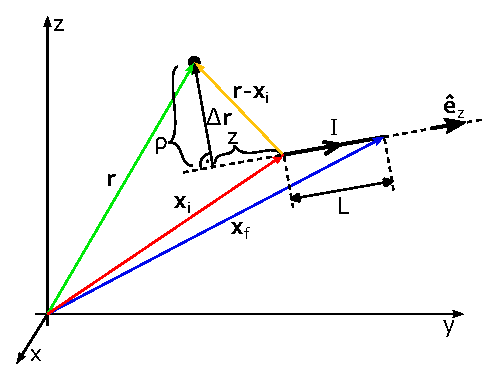
\includegraphics{img/StraightWireSegment_MappingToCartesian.eps}
 \caption{Mapping the components to global coordinates for an exemplary straight wire segment.
          The wire segment is positioned from~$\mathbf{x}_\mathrm{i}$ to~$\mathbf{x}_\mathrm{f}$.
          Its parallel unit vector is denoted $\hat{\mathbf{e}}_z$.
          The length of the wire segment is denoted by~$L$.
          The evaluation location is denoted by~$\mathbf{r}$.}
 \label{fig:StraightWireSegment_MappingToCartesian}
\end{figure}
The length of the wire segment is denoted by~$L$:
\begin{equation}
  L = |\mathbf{x}_f - \mathbf{x}_i| \, .
\end{equation}
If $L=0$, no contribution is taken into account from the wire segment.
Otherwise, the unit vector along the segment~$\hat{\mathbf{e}}_z$ is computed as:
\begin{equation}
  \hat{\mathbf{e}}_z = \frac{\mathbf{x}_f - \mathbf{x}_i}{L} \, .
\end{equation}
The vertical coordinate~$z$ in the coordinate system of the wire segment is:
\begin{equation}
  z = (\mathbf{r} - \mathbf{x}_i) \cdot \hat{\mathbf{e}}_z
\end{equation}
and the normalized $z$-coordinate is:
\begin{equation}
  z' = \frac{z}{L} = \frac{1}{L} (\mathbf{r} - \mathbf{x}_i) \cdot \hat{\mathbf{e}}_z \, .
\end{equation}
For the radial coordinate, first the vector~$\Delta \mathbf{r}$ is formed:
\begin{equation}
  \Delta \mathbf{r} = (\mathbf{r} - \mathbf{x}_i) - z \, \hat{\mathbf{e}}_z
\end{equation}
and the radial coordinate $\rho$ is then obtained by taking $\rho = |\Delta \mathbf{r}|$.
The normalized radial coordinate~$\rho'$ is then obtained as:
\begin{equation}
  \rho' = \frac{\rho}{a} = \frac{1}{a} |(\mathbf{r} - \mathbf{x}_i) - z \, \hat{\mathbf{e}}_z| \, .
\end{equation}
The magnetic vector potential only has a component in parallel direction in the coordinate system of the wire segment.
The vector potential of the circular wire loop in thus in Cartesian coordinates:
\begin{equation}
  \mathbf{A}(\mathbf{r}) = A_z(\rho', z') \hat{\mathbf{e}}_z \, .
\end{equation}
If $\rho' \neq 0$, a unit vector in radial direction is formed as follows:
\begin{equation}
  \hat{\mathbf{e}}_\rho = \frac{\Delta \mathbf{r}}{\rho}
\end{equation}
and the magnetic field of the straight wire segment (consisting only of the tangential component~$B_\varphi$)
is evaluated as:
\begin{equation}
  \mathbf{B}(\mathbf{r}) = B_\varphi(\rho', z') \hat{\mathbf{e}}_\varphi
\end{equation}
with $\hat{\mathbf{e}}_\varphi = \hat{\mathbf{e}}_z \times \hat{\mathbf{e}}_\rho$.

\subsubsection{Circular Wire Loop}
Figure~\ref{fig:CircularWireLoop_MappingToCartesian} illustrates the setup of a circular wire loop.
\begin{figure}[htbp]
 \centering
 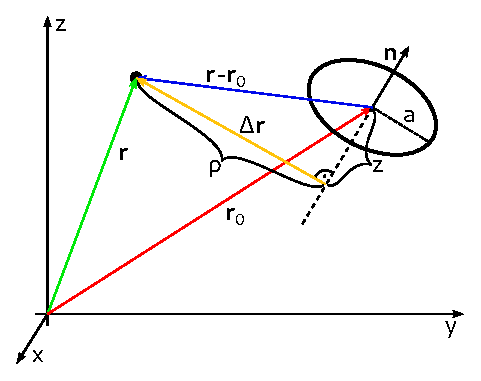
\includegraphics{img/CircularWireLoop_MappingToCartesian.eps}
 \caption{Mapping the components to Cartesian coordinates for an exemplary circular wire loop.
          The loop is centered around its origin~$\mathbf{r}_0$.
          Its normal vector is denoted $\mathbf{n}$ and defines the orientation of the loop.
          The radius of the loop is denoted by~$a$.
          The evaluation location is denoted by~$\mathbf{r}$.}
 \label{fig:CircularWireLoop_MappingToCartesian}
\end{figure}
The $z$-axis of the coordinate system of the wire loop is defined by the normal vector~$\mathbf{n}$:
\begin{equation}
  \hat{\mathbf{e}}_z = \frac{\mathbf{n}}{|\mathbf{n}|} \, .
\end{equation}
The $z$ component of the evaluation location is thus obtained as follows:
\begin{equation}
  z = (\mathbf{r} - \mathbf{r}_0) \cdot \hat{\mathbf{e}}_z \, .
\end{equation}
The normalized $z$-coordinate $z'$ is then obtained as:
\begin{equation}
  z' = \frac{z}{a} = \frac{1}{a} (\mathbf{r} - \mathbf{r}_0) \cdot \hat{\mathbf{e}}_z \, .
\end{equation}
For the radial coordinate, first the vector~$\Delta \mathbf{r}$ is formed:
\begin{equation}
  \Delta \mathbf{r} = (\mathbf{r} - \mathbf{r}_0) - z \, \hat{\mathbf{e}}_z
\end{equation}
and the radial coordinate $\rho$ is then obtained by taking $\rho = |\Delta \mathbf{r}|$.
The normalized radial coordinate~$\rho'$ is then obtained as:
\begin{equation}
  \rho' = \frac{\rho}{a} = \frac{1}{a} |(\mathbf{r} - \mathbf{r}_0) - z \, \hat{\mathbf{e}}_z| \, .
\end{equation}
The magnetic field of the circular wire loop consists of two cylindrical components, namely $B_\rho$ and $B_z$.
The Cartesian magnetic field components are then computed as follows:
\begin{equation}
  \mathbf{B}(\mathbf{r}) = B_\rho(\rho', z') \hat{\mathbf{e}}_\rho + B_z(\rho', z') \hat{\mathbf{e}}_z \, .
\end{equation}
If $\rho' = 0$, only $B_z$ is evaluated.
Otherwise, a unit vector in radial direction is formed as follows:
\begin{equation}
  \hat{\mathbf{e}}_\rho = \frac{\Delta \mathbf{r}}{\rho}
\end{equation}
and $B_\rho$ is evaluated as well.
The magnetic vector potential only has a component in tangential direction in the coordinate system of the wire loop.
It is also only evaluated if $\rho' \neq 0$.
The corresponding unit vector~$\hat{\mathbf{e}}_\varphi$ is then given by
$\hat{\mathbf{e}}_\varphi = \hat{\mathbf{e}}_z \times \hat{\mathbf{e}}_\rho$.
The vector potential of the circular wire loop in thus in Cartesian coordinates:
\begin{equation}
  \mathbf{A}(\mathbf{r}) = A_\varphi(\rho', z') \hat{\mathbf{e}}_\varphi \, .
\end{equation}

\FloatBarrier
\subsection{Verification Method}
\label{sec:methods_verification}
The implementations of above formulas for the magnetic vector potential
and magnetic field of a straight wire segment and a circular wire loop
need to be tested before using the implementations in routine work.
This section introduces the choice of test point coordinates.
A rectangular grid of test points in the $(\rho', z')$-plane is defined,
where the choice of knots along the $\rho'$ and $z'$ axes are discussed below.
The set of test point coordinates for testing a given current carrier primitive
consists of the combinations of all test knots along the $\rho'$ axis
with all test knots along the $z'$ axis.
Let $T_{\rho'}$ ($T_{z'}$) be the set of knots along the $\rho'$ ($z'$) axis to test the formulation on.
Then $T = T_{\rho'} \otimes T_{z'} \\ T_\mathrm{cc}$ is the set of test point coordinates
where $\otimes$ is the cartesian product of two sets
and $T_\mathrm{cc}$ is the subset of points from $T_{\rho'} \otimes T_{z'}$ that are located exactly on the current carrier.
First, the choice of test points for testing the implementations
of the straight wire segment methods~(SWS) is introduced.
The set of grid knots along the $\rho'$ axis, $T^\mathrm{SWS}_{\rho'}$, are chosen as follows:
\begin{itemize}
  \item $T^\mathrm{SWS}_{\rho',1} = \{ 0 \}$
  \item $T^\mathrm{SWS}_{\rho',2} = \{ 10^{-30}, 10^{-29}, ..., 10^{30} \}$
\end{itemize}
with $T^\mathrm{SWS}_{\rho'} = T^\mathrm{SWS}_{\rho',1} \cup T^\mathrm{SWS}_{\rho',2}$,
leading to $|T^\mathrm{SWS}_{\rho'}| = 62$.
The set of grid knots along the $z'$ axis, $T^\mathrm{SWS}_{z'}$, are chosen as follows:
\begin{itemize}
  \item $T^\mathrm{SWS}_{z',1} = \{ -10^{30}, -10^{29}, ..., -10^{-30} \}$
  \item $T^\mathrm{SWS}_{z',2} = \{ 10^{-30}, 10^{-29}, ..., 10^{-1} \}$
  \item $T^\mathrm{SWS}_{z',3} = \{ 1 - 10^{-1}, 1 - 10^{-2}, ..., 1 - 10^{-15}, 1 - \epsilon_{64}/2 \}$
  \item $T^\mathrm{SWS}_{z',4} = \{ 1 + \epsilon_{64}, 1 + 10^{-15}, 1 + 10^{-14}, ..., 1 + 10^{-1} \}$
  \item $T^\mathrm{SWS}_{z',5} = \{ 10^{1}, 10^{2}, ..., 10^{30} \}$
  \item $T^\mathrm{SWS}_{z',6} = \{ 0, 1/2, 1, 2 \}$
\end{itemize}
with $T^\mathrm{SWS}_{z'} = T^\mathrm{SWS}_{z',1} \cup T^\mathrm{SWS}_{z',2} \cup T^\mathrm{SWS}_{z',3} \cup T^\mathrm{SWS}_{z',4} \cup T^\mathrm{SWS}_{z',5} \cup T^\mathrm{SWS}_{z',6}$,
leading to $|T^\mathrm{SWS}_{z'}| = 157$.
The machine-precision epsilon is given by $\epsilon_{64} \approx 2.2 \times 10^{-16}$ for the case of \texttt{binary64}.
The exclusion of the test points that are located exactly on the wire segment leads to
a total number of test point coordinates~$T_\mathrm{SWS}$ for the straight wire segment of
$|T_\mathrm{SWS}| = 9685$.
Next, the choice of test points for testing the implementations
of the circular wire loop~(CWL) methods is introduced.
The set of grid knots along the $\rho'$ axis, $T^\mathrm{CWL}_{\rho'}$, are chosen as follows:
\begin{itemize}
  \item $T^\mathrm{CWL}_{\rho',1} = \{ 10^{-30}, 10^{-29}, ..., 10^{-1} \}$
  \item $T^\mathrm{CWL}_{\rho',2} = \{ 1 - 10^{-1}, 1 - 10^{-2}, ..., 1 - 10^{-15}, 1 - \epsilon_{64}/2 \}$
  \item $T^\mathrm{CWL}_{\rho',3} = \{ 1 + \epsilon_{64}, 1 + 10^{-15}, 1 + 10^{-14}, ..., 1 + 10^{-1} \}$
  \item $T^\mathrm{CWL}_{\rho',4} = \{ 10^{1}, 10^{2}, ..., 10^{30} \}$
  \item $T^\mathrm{CWL}_{\rho',5} = \{ 0, 1/2, 1, 2 \}$
\end{itemize}
with $T^\mathrm{CWL}_{\rho'} = T^\mathrm{CWL}_{\rho',1} \cup T^\mathrm{CWL}_{\rho',2} \cup T^\mathrm{CWL}_{\rho',3} \cup T^\mathrm{CWL}_{\rho',4} \cup T^\mathrm{CWL}_{\rho',5}$,
leading to $|T^\mathrm{CWL}_{\rho'}| = 96$.
The set of grid knots along the $z'$ axis, $T^\mathrm{CWL}_{z'}$, are chosen as follows:
\begin{itemize}
  \item $T^\mathrm{CWL}_{z',1} = \{ 0 \}$
  \item $T^\mathrm{CWL}_{z',2} = \{ 10^{-30}, 10^{-29}, ..., 10^{30} \}$
\end{itemize}
with $T^\mathrm{CWL}_{z'} = T^\mathrm{CWL}_{z',1} \cup T^\mathrm{CWL}_{z',2}$,
leading to $|T^\mathrm{CWL}_{z'}| = 62$.
The exclusion of the test point that is located exactly on the wire loop leads to
a total number of test point coordinates~$T_\mathrm{CWL}$ for the circular wire loop of
$|T_\mathrm{CWL}| = 5951$.
The reference results are computed on each test point using arbitrary-precision arithmetic
as provided by the Python package~\texttt{mpmath}~\cite{mpmath} and Mathematica~\cite{Mathematica}.
The test point coordinates are computed within the finite-precision test programs used to check the accuracy of the results.
This implies that the exact \textit{implied} values of the test point coordinates have to be transported
into the arbitrary-precision software used to compute the reference data.
The evaluation positions are specified at IEEE754~\texttt{binary64} floating-point numbers.
The floating point numbers are re-constructed within the arbitrary-precision software
in order to properly transport their intended value.
In case of \texttt{binary64}, this is done as follows for a floating-point number~$f$:
\begin{equation}
 f(s, E, M) =
 \begin{cases}
   0                                                             &: E=0 \textrm{ and } M=0 \\
   (-1)^s \, 2^{E - 1023} \, \left( 1 + \frac{M}{2^{52}} \right) &: \textrm{else}
  \end{cases} \label{eqn:binary64}
\end{equation}
where $s$ is the sign bit, $E$ is the exponent specified as an 11-bit unsigned integer
and $M$ is the mantissa specified as a 52-bit unsigned integer.
Several special cases are defined for certain values of $s$, $E$ and $M$,
but in the context of this work only the case $E=0$, $M=0$ ($s$ arbitrary),
which represents an exact zero, is relevant.
The organization of those bits in a \texttt{binary64} number is shown in Fig.~\ref{fig:binary64}.
\begin{figure}[htbp]
 \centering
 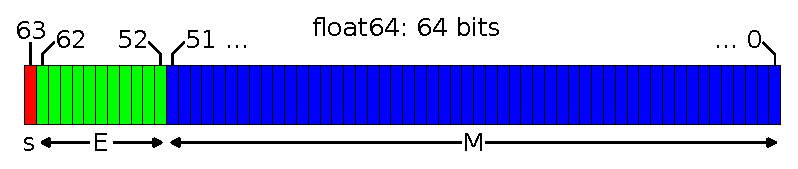
\includegraphics{img/IEEE754_binary64.eps}
 \caption{Organization of sign bit~$s$, exponent~$E$ (11 bits, unsigned integer)
          and mantissa~$M$ (52 bits, unsigned integer) within the 64 bits
          of a IEEE754~\texttt{binary64} floating-point number.
          Each box represents one bit and the colors indicate which quantity a bit belongs to
          (red: sign bit, green: exponent, blue: mantiassa).}
 \label{fig:binary64}
\end{figure}
In particular, a test point coordinate value~$f$ is passed to the reference computation
by passing the three values $s$, $E$ and $M$ as integers (which are easy to represent exactly).
Within the reference computation, the value of $f$ is constructed using~\eqn{binary64} implemented
in arbitrary precision and with the exact values of $s$, $E$ and $M$.
The reference data for the straight wire segment methods
is computed using 300 decimal digits of precision.
The reference data for the circular wire loop
is computed using 200 decimal digits of precision.
The evaluation position is specified exactly
via $s_\rho$, $E_\rho$ and $M_\rho$ (for $\rho'$)
and $s_z$, $E_z$ and $M_z$ (for $z'$):
\begin{align}
 \rho' \leftarrow&\, \begin{cases}
                       0  &:\, E_\rho = 0 \textrm{ and } M_\rho = 0 \\
                       (-1)^{s_\rho} \, 2^{E_\rho - 1023} \, \left(1 + M_\rho / 2^{52}  \right) &:\, \textrm{else}
                     \end{cases} \nonumber \\
    z' \leftarrow&\, \begin{cases}
                       0  &:\, E_z = 0 \textrm{ and } M_z = 0 \\
                       (-1)^{s_z   } \, 2^{E_z    - 1023} \, \left(1 + M_z / 2^{52}  \right) &:\, \textrm{else}
                     \end{cases} \nonumber
\end{align}
The following algorithm is used to compute reference values
of $\tilde{A}_z$ and $\tilde{B}_\varphi$ at~$(\rho', z')$
for the straight wire segment:
\begin{align}
  r_\mathrm{i}  \leftarrow&\, \sqrt{ {\rho'}^2 + {z'}^2 } \nonumber \\
  r_\mathrm{f}  \leftarrow&\, \sqrt{ {\rho'}^2 + \left(1 - z'\right)^2 } \nonumber \\
  \epsilon \leftarrow&\, \left( r_\mathrm{i} + r_\mathrm{f} \right)^{-1} \nonumber \\
  \tilde{A}_z \leftarrow&\, \textrm{atanh} (\epsilon) \label{eqn:sws_A_z_ref} \\
  \tilde{B}_\varphi \leftarrow&\, \left(\frac{1}{r_\mathrm{i}} + \frac{1}{r_\mathrm{f}} \right) \frac{\rho'}{r_\mathrm{i} r_\mathrm{f} + {\rho'}^2 + z' (z' - 1)} \label{eqn:sws_B_phi_ref}
\end{align}
The following algorithm is used to compute reference values
of $\tilde{A}_\varphi$ and $\tilde{B}_\rho$ at~$(\rho', z')$
for the circular wire loop:
\begin{align}
 k_c^2 \leftarrow&\, \frac{{z'}^2 + \left(1 - \rho'\right)^2}{{z'}^2 + \left(1 + \rho'\right)^2} \nonumber \\
 \tilde{A}_\varphi \leftarrow&\,
 \begin{cases}
   0 &:\, \rho' = 0 \\
   \frac{1}{\sqrt{{z'}^2 + \left(1 + \rho'\right)^2}}
                                 \int\limits_0^{\pi/2}
                                   \frac{\sin^2(\varphi) - \cos^2(\varphi)}
                                        {\sqrt{\cos^2(\varphi) + k_c^2 \sin^2(\varphi)}} \,\mathrm{d}\varphi &:\, \textrm{else}
 \end{cases} \label{eqn:A_phi_ref} \\
 \tilde{B}_\rho \leftarrow&\,
 \begin{cases}
   0 &:\, \rho' = 0 \textrm{ or } z' = 0 \\
   \frac{z'}{\left[{z'}^2 + \left(1 + \rho'\right)^2\right]^{3/2}}
                                 \int\limits_0^{\pi/2}
                                   \frac{\sin^2(\varphi) - \cos^2(\varphi)}
                                        {\left[\cos^2(\varphi) + k_c^2 \sin^2(\varphi)\right]^{3/2}} \,\mathrm{d}\varphi &:\, \textrm{else}
 \end{cases} \label{eqn:B_rho_ref}
\end{align}
The method used to compute $\tilde{B}_z$ works slightly differently:
\begin{align}
 k^2 \leftarrow&\,
  \begin{cases}
    4 / \left( \frac{1}{\rho'} + 2 + \rho' \right)    &: z' = 0 \\
    \frac{4 \rho'}{{z'}^2 + \left(1 + \rho'\right)^2} &: \textrm{else}
  \end{cases} \nonumber \\
 \tilde{B}_z \leftarrow&\,
   \frac{1}{\left[ {z'}^2 + \left(1 + \rho'\right)^2 \right]^{3/2} }
                                 \int\limits_0^{\pi/2}
                                   \frac{(1-\rho') \sin^2(\varphi) + (1+\rho') \cos^2(\varphi)}
                                        {\left[1 - k^2 \sin^2(\varphi) \right]^{3/2}} \,\mathrm{d}\varphi  \label{eqn:B_z_ref}
\end{align}
The integrals are carried out numerically within the arbitrary-precision software.
In case of~\texttt{mpmath}, double-exponential quadrature~\cite{double_exp_quad} is used~\cite{mpmath_quad}.
The particular choices for the number of digits of precision used throughout the arbitrary-precision computation
mentioned above have been adjusted to robustly yield enough equal digits
in the outputs from \texttt{mpmath} and Mathematica for benchmarking the \texttt{binary64} implementation of the methods presented in Sec.~\ref{sec:methods_sws} and~\ref{sec:methods_cwl}.
The error metric employed in this work is given as follows:
\begin{equation}
 \delta(a, b)
 = \begin{cases}
    \log_{10} \left(\min\left(1, \left| \frac{a - b}{b} \right|\right) \right) &: b \neq 0, a \neq b \\
    0                                                                          &: b=0, a \neq 0 \\
    -16                                                                        &: \textrm{else}
   \end{cases} \label{eqn:error_metric}
\end{equation}
where the constant~$-16$ is chosen for \texttt{binary64} as $\lfloor \log_{10}(\epsilon_{64}) \rfloor$.
Here, $a$ is the value to be tested and
$b$ is the reference value computed using arbitrary-precision arithmetic.
